\documentclass[pdftex]{beamer}
\usepackage[ruled]{algorithm2e}
\usepackage{algorithmic}
%\usetheme{Frankfurt}

% declare the path(s) where your graphic files are
% ../.. is the GeocronDocuments directory
\graphicspath{{../../images/diagrams/}}
\DeclareGraphicsExtensions{.pdf,.png}

\begin{document}

\title[Short Title]{Simulating Disaster Scenarios and Geographically-Correlated Resilient Overlay Networks}
\subtitle{Heuristics for Location-based Routing}
\author[K. Benson and Z. Huang]{Kyle E. Benson and Zhipeng Huang}
\institute[UCI]{
  Department of Computer Science\\
  University of California, Irvine\\
  Irvine, California 92697\\[1ex]
  \texttt{kebenson@uci.edu} and \texttt{zhipengh@uci.edu}
}

% % % % % % % % % % % % % % % % % % % % % % % % % % % % % % % % % % % % % % % % % %

\begin{frame}[plain]
	\titlepage
\end{frame}

% % % % % % % % % % % % % % % % % % % % % % % % % % % % % % % % % % % % % % % % % %

\begin{frame}{Orthogonal Distant Path Heuristic}
\begin{columns}
\begin{column}{.5\textwidth}

% re-works this itemize into a different background slide.
% put algorithm here instead, maybe an observation/intuition

\begin{itemize}
	\item Failure along path to server or in local area
	\item Choose node outside local	region to avoid overlapping	paths
	\item Choose path avoiding as much of the direct path as possible
	\item Overlay node may use similar route to sensor
\end{itemize}
\end{column}
	
\begin{column}{.5\textwidth}
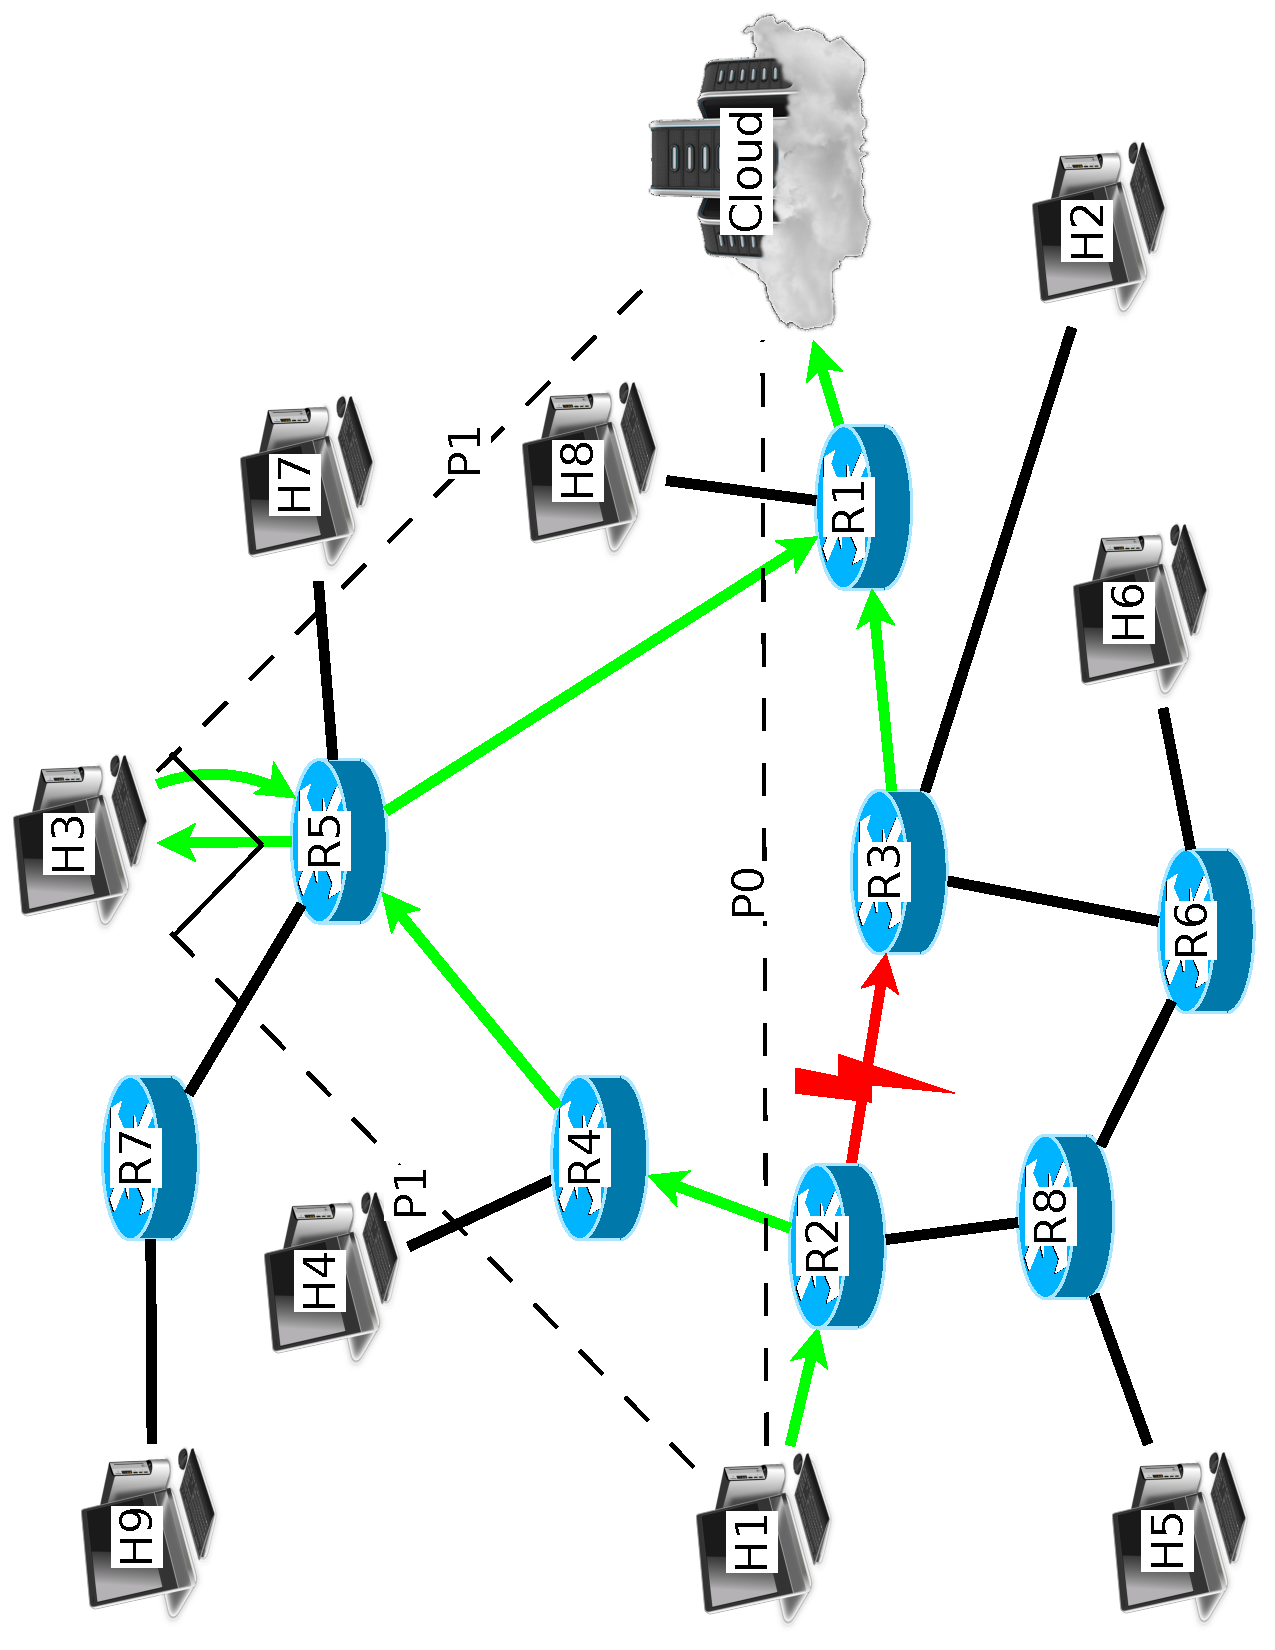
\includegraphics[height=\textwidth,angle=-90]{angular_path}
\end{column}

\end{columns}
\end{frame}


% % % % % % % % % % % % % % % % % % % % % % % % % % % % % % % % % % % % % % % % % %
\begin{frame}{Angle-Dependent Path Heuristic}
\begin{columns}

\begin{column}{.5\textwidth}
\begin{algorithm}[H]
\DontPrintSemicolon
\SetKwBlock{Begin}{begin}{end}
\SetAlgoLined
\SetAlgoLongEnd
\scriptsize
\Begin{
\tcc*[l]{For angle-dependent path heuristic algorithm.}
\lIf{$angle = \pi$ {\bf or} $angle = 0$} {$likelihood = 0$\;}
\lElseIf{$angle < \pi$} {$likelihood = \cos (angle - 0.25 \cdot \pi)$\;}
\lElseIf{$angle > \pi$} {$likelihood = \cos (2 \cdot ((2 \cdot \pi - angle) - 0.25 \cdot \pi)/3)$\;}
}
\caption{Angle-Dependent Path Heuristic Algorithms}
\small
\end{algorithm}
\end{column}
	
\begin{column}{.5\textwidth}
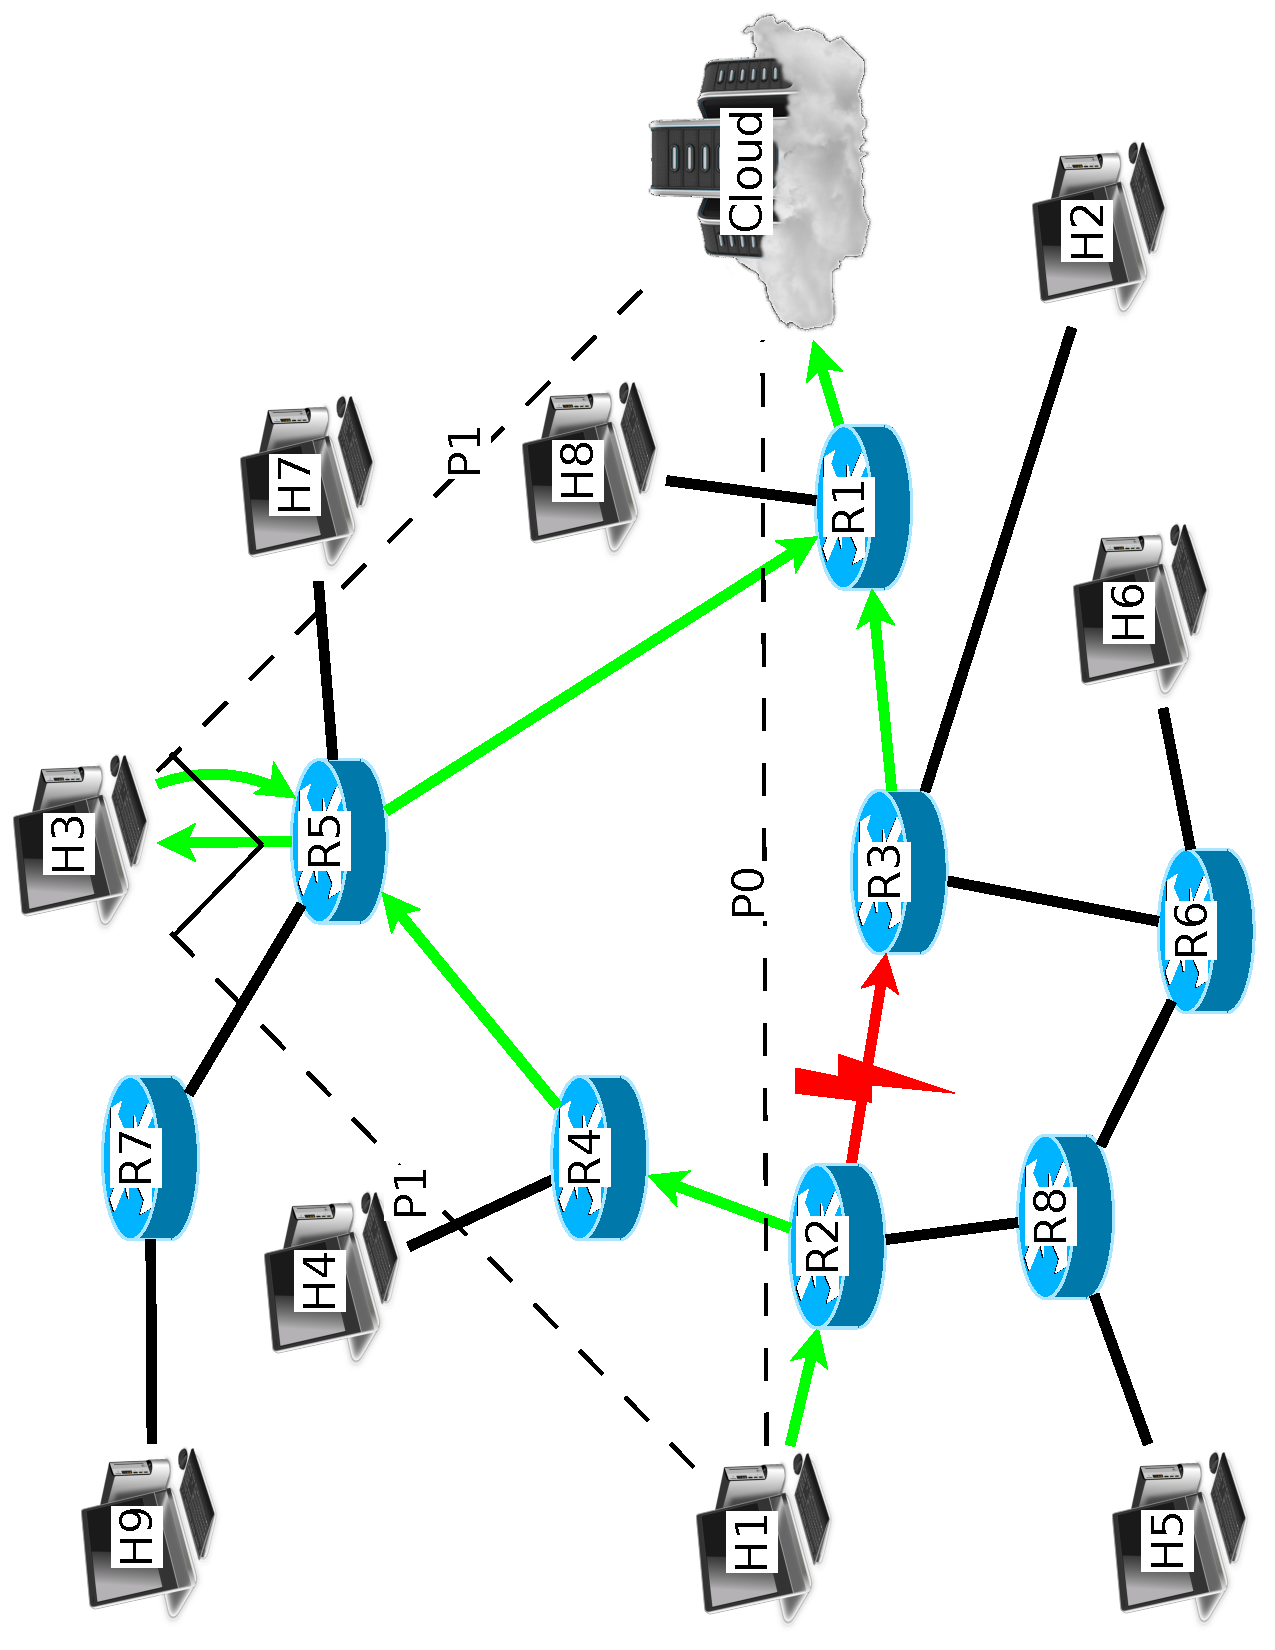
\includegraphics[height=\textwidth,angle=-90]{angular_path}
\end{column}

\end{columns}
\end{frame}

% % % % % % % % % % % % % % % % % % % % % % % % % % % % % % % % % % % % % % % % % %

\begin{frame}{Distance-Dependent Path Heuristic}
\begin{columns}
\begin{column}{.5\textwidth}
\begin{algorithm}[H]
\DontPrintSemicolon
\SetKwBlock{Begin}{begin}{end}
\SetAlgoLined
\SetAlgoLongEnd
\scriptsize
%\SetAlgoSkip{bigskip}
%\SetAlgoInsideSkip{medskip}
%$/*Initialization*/$\;
\Begin{
\tcc*[l]{For distance-dependent path heuristic algorithm.}
\lIf{$distance < minDistance$} {$likelihood = 0$\;}
\lElseIf{$minDistance < distance < mDistance$} {$likelihood = 0.4 \cdot (distance - minDistance)$\;}
\lElseIf{$mDistance < distance < maxDistance$} {$llikelihood = (distance - minDistance)$\;}
\lElseIf{$distance > maxDistance$} {$likelihood = 0.8 \cdot (distance - minDistance)$\;}
}
\caption{Distance-Dependent Path Heuristic Algorithms}
\small
\end{algorithm}
\end{column}
	
\begin{column}{.5\textwidth}
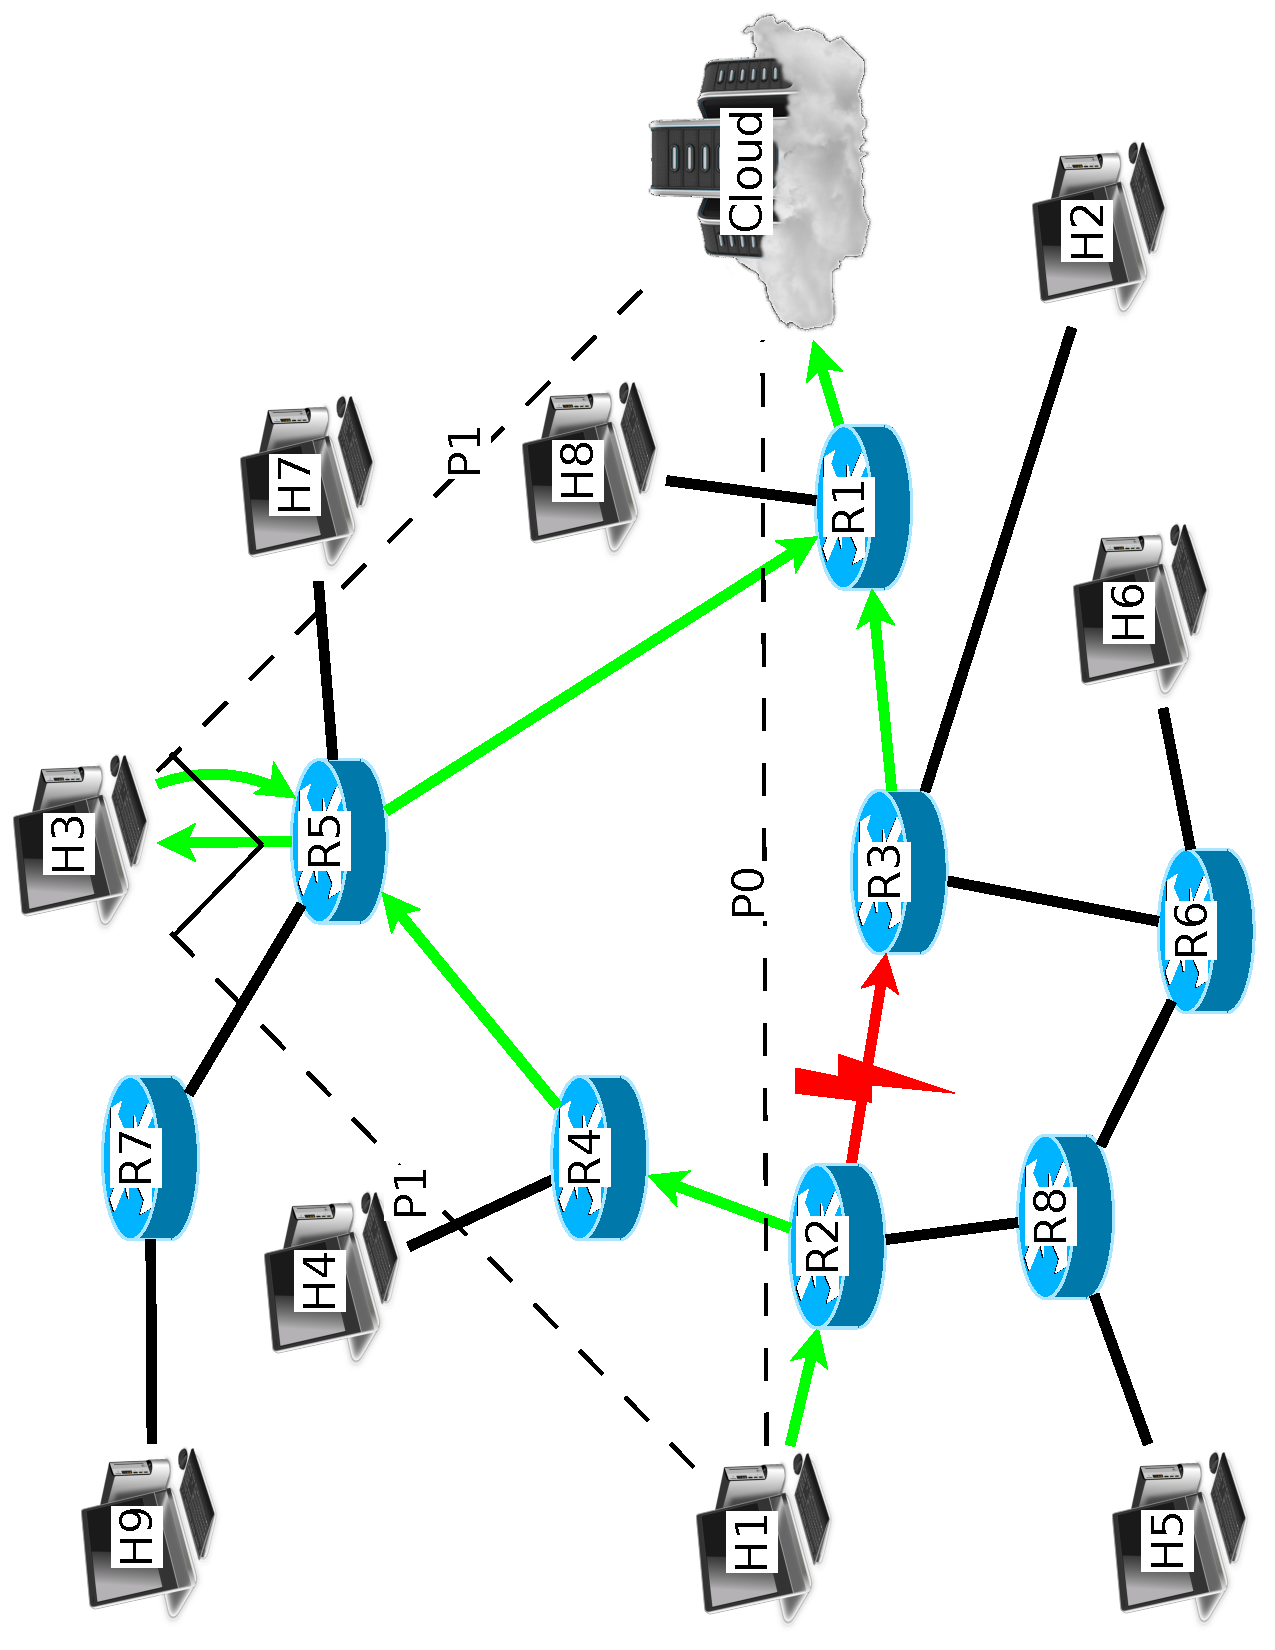
\includegraphics[height=\textwidth,angle=-90]{angular_path}
\end{column}

\end{columns}
\end{frame}

% % % % % % % % % % % % % % % % % % % % % % % % % % % % % % % % % % % % % % % % % %

\begin{frame}{Furthest Distant Path Heuristic}
\begin{columns}
\begin{column}{.5\textwidth}
\begin{itemize}
	\item Failure along path to server or in local area
	\item Choose node that has the largest distance from the source
	\item Choose path avoiding as much of the direct path as possible
	\item Overlay node may use similar route to sensor
\end{itemize}
\end{column}
	
\begin{column}{.5\textwidth}
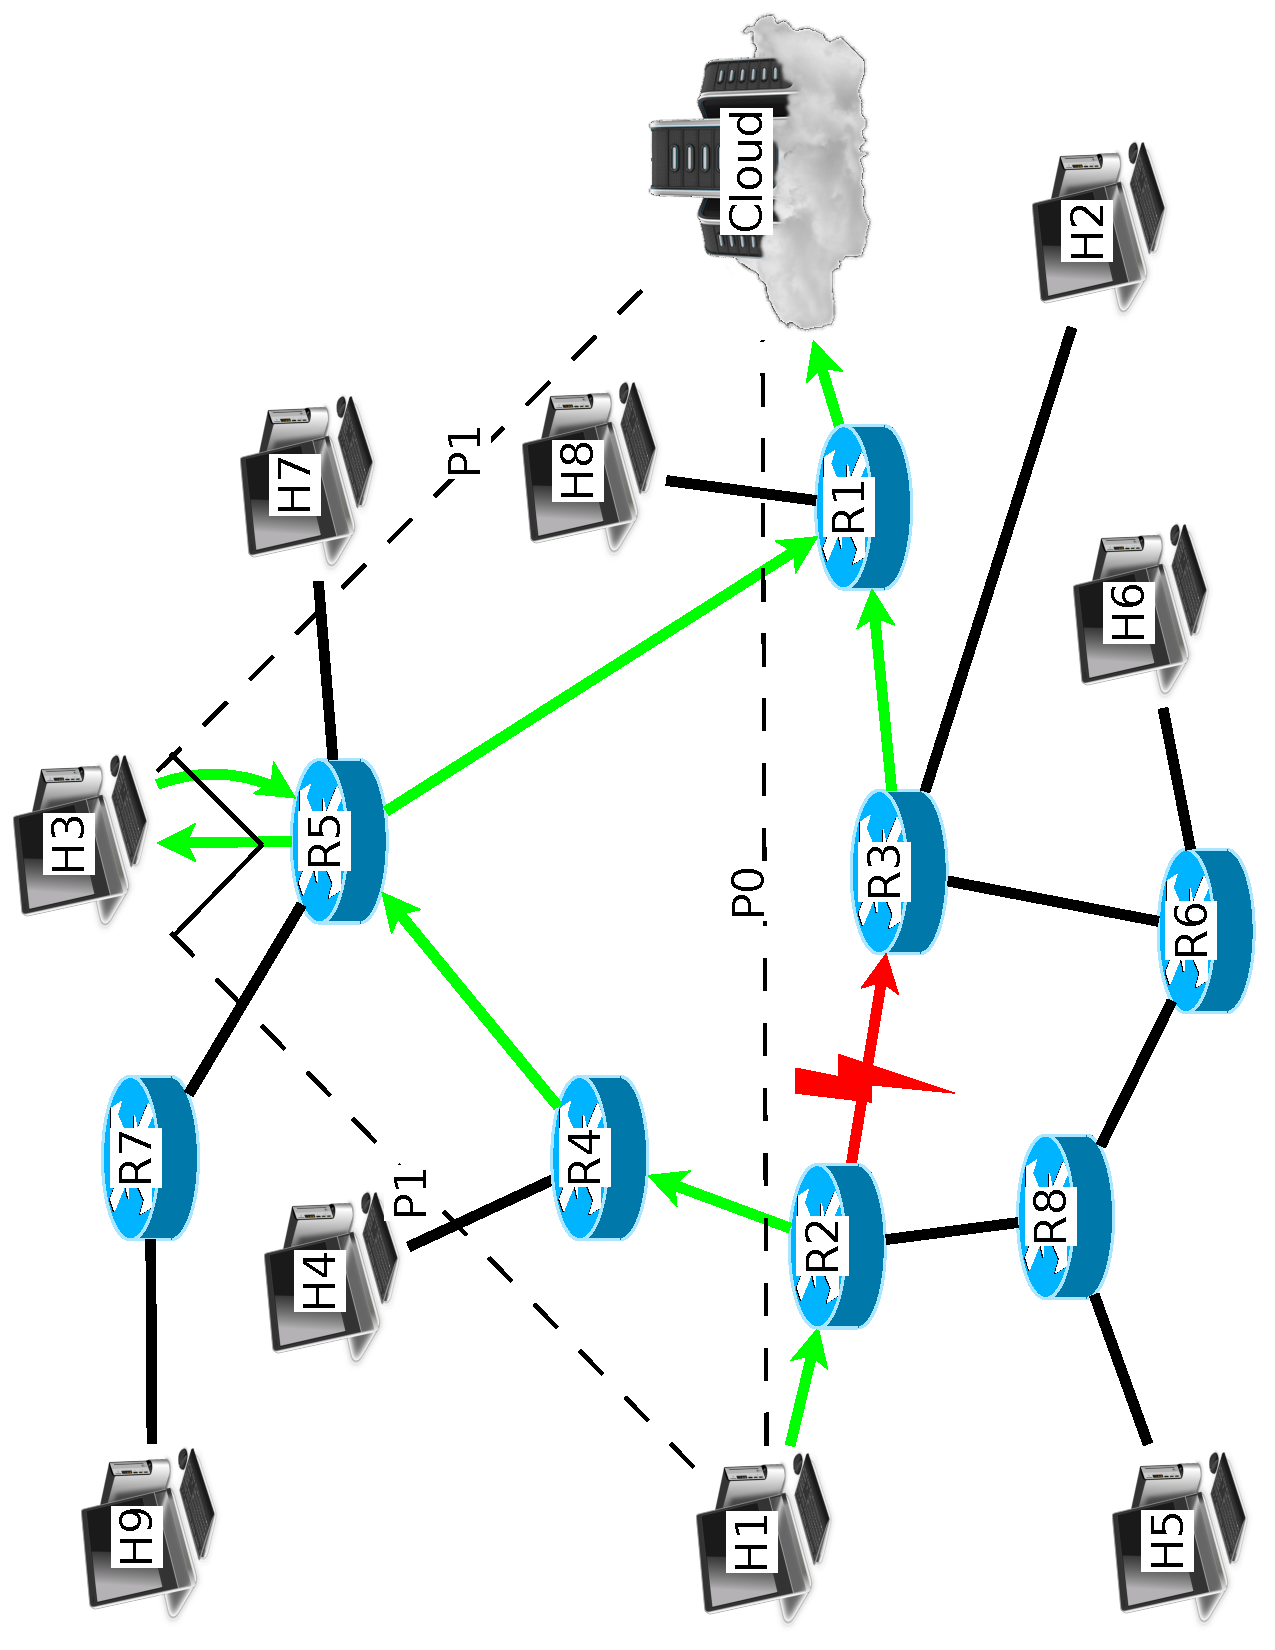
\includegraphics[height=\textwidth,angle=-90]{angular_path}
\end{column}

\end{columns}
\end{frame}


%
%\part{rest}
%
%\begin{frame}{Roadmap}
%	\tableofcontents
%\end{frame}
%
%\section{Location Service}
%
%\begin{frame}{Location Service}
%\begin{columns}
%\begin{column}{.5\textwidth}
%
%	\begin{itemize}
%		\item Nodes have GPS
%		\item But how to look up destination's location?
%		\item Maintain global information \uncover<2->{\alert{easily outdated/inefficient}}
%		\item<3-> Distribute load
%		\begin{itemize}
%			\item In , node updates \emph{location servers} (LS) throughout network
%			\item Divide network into hierarchical grid
%			\item LS's in 3 external grids at each level
%			\item Lookup distance $<$ square LS co-resides in
%		\end{itemize}
%		
%	\end{itemize}
%
%\end{column}
%
%\begin{column}{.5\textwidth}
%\uncover<3->{
%\begin{figure}
%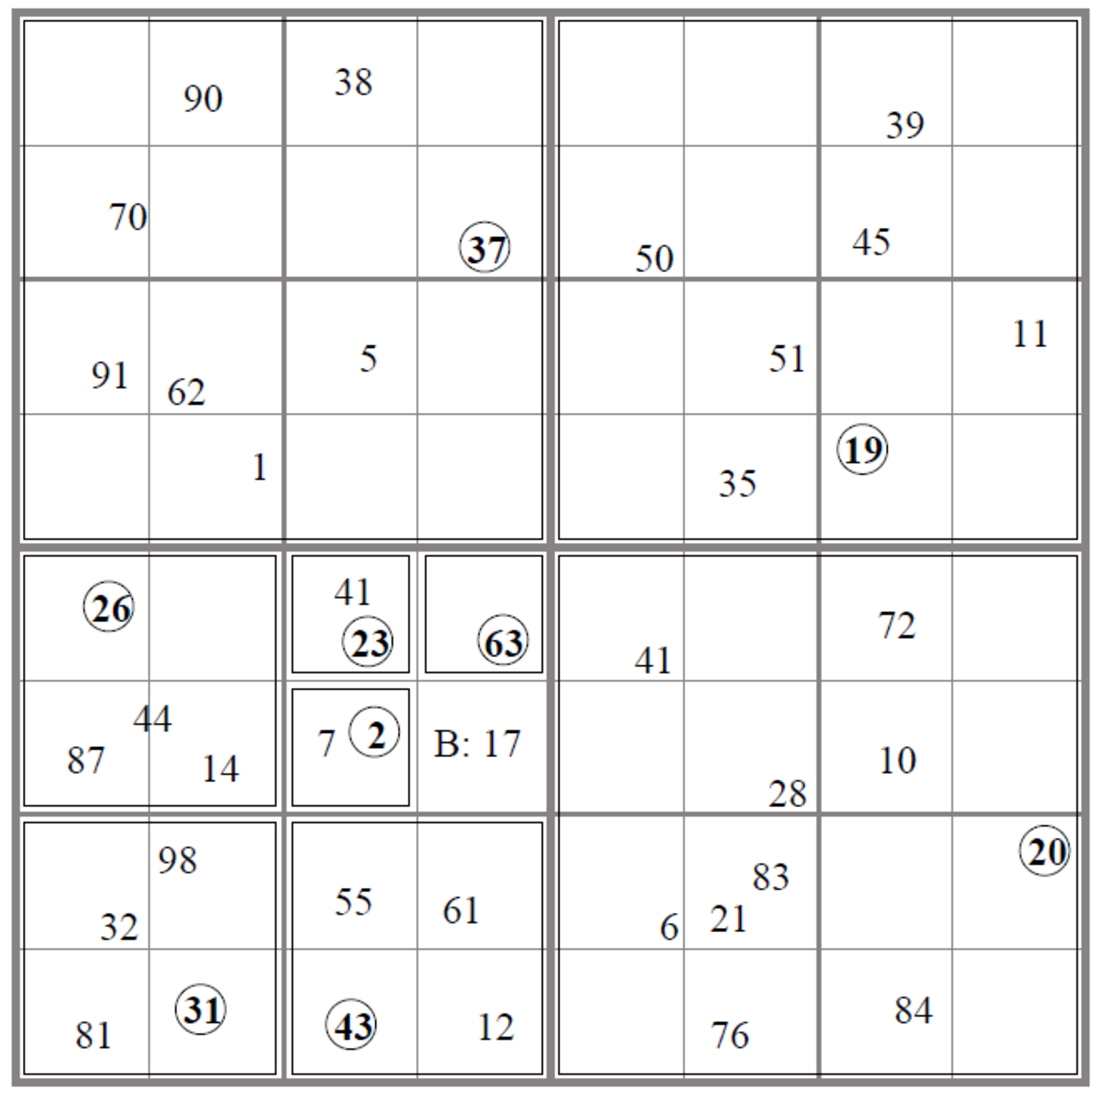
\includegraphics[width=\textwidth]{location_service}
%\caption{Hierarchical grid with 4 order-i squares in order-i+1 square.}
%\end{figure}}
%\end{column}
%\end{columns}
%\end{frame}
%

\end{document}
